\chapter{Военные корабли и их операторы}
\label{ch:ships-chapter}

Глава посвящена отечественным и зарубежным кораблям. 
Они могут иметь как военное, так~и~гражданское назначение. 
Гражданские суда используются в грузоперевозках, рыболовстве, туризме, 
разведке полезных ископаемых, спасательных работах, 
а также в~спортивных, культурных и других целях. 
Для~хранения информации о судах и других объектах ведутся базы знаний. 
Одной из таких баз знаний являются Викиданные. 
В этой главе изучены хранимые в Викиданных объекты кораблей и проведена оценка качества и полноты их описания.


\begin{marginfigure}[0.0cm]
  \includegraphics[width=0.9\linewidth]{chapter/ship/Russian_ships_topic_imbalance.png}
  \caption{Индекс Джини~--- равномерность заполнения свойств <<кораблей>>,\\
           2020 год}
  \label{fig:prowd_ships-unbalanced}%
\end{marginfigure}


\section{Список кораблей}

\index{Коэффициент Джини}
Анализ экземпляров объекта \wdqName{корабль}{11446} 
с~помощью сервиса ProWD в~2020 году показал, 
что индекс Джини равен 0.239 (рис.~\ref{fig:prowd_ships-unbalanced}). 
%
Сравнение кораблей со странами в Викиданных 
(у стран индекс Джини равен 0.091, см. рис.~\ref{fig:ProWD_country} 
                                  на~с.~\pageref{fig:ProWD_country}) 
говорит, что корабли не так хорошо и равномерно заполнены, как~страны, 
есть достаточно кораблей как с~большим количеством заполненных свойств, 
так и с малым.

%Итак, кроме объекта \wdqName{корабль}{11446} нам потребуются свойства:
%   \wdProperty{31}{экземпляр}, 
%   \wdProperty{137}{оператор}, 
%   \wdProperty{17}{государство} и  
%   \wdProperty{607}{конфликт}.
Построим список всех кораблей с помощью запроса~\ref{lst:ships_ru}.


\begin{lstlisting}[ language=SPARQL, 
            caption={{\href{https://w.wiki/wX6}{Список кораблей}}\protect\footnotemark}, 
            label=lst:ships_ru, 
            numbers=none
            ]
# List of ships
SELECT ?ship ?shipLabel WHERE {
  ?ship wdt:P31 wd:Q11446. # instance of ship
  SERVICE wikibase:label {bd:serviceParam wikibase:language "ru, en"}
}
\end{lstlisting}
\footnotetext{Получено: \num{19820} кораблей в~2017 году, 
                        \num{50681}~--- в~2020-м, 
                        \num{71203}~--- в~2021 году. 
        Ссылка на~SPARQL-запрос: \href{https://w.wiki/wX6}{https://w.wiki/wX6}.}


\newpage
По данным ProWD, больше всего свойств (34 свойства) имеет 
\href{https://www.wikidata.org/wiki/Q281147}{ледокол <<Красин>> (Q281147)}, 
а~меньше всего, по~пять свойств, у~кораблей 
\href{https://www.wikidata.org/wiki/Q99198666}{<<Ливень>> (Q99198666)} и 
\href{https://www.wikidata.org/wiki/Q28155282}{Dispatch (Q28155282)}.

В Викиданных, как правило, записывается не прямая принадлежность корабля стране, 
а~принадлежность некоторому оператору. 
Чаще всего это какая-либо организация, 
например 
\wdqName{Военно-морской флот Российской Федерации}{465283}.\, 
Составим список кораблей, 
операторы которых находятся или~находились в России, СССР или Российской империи 
(см. запрос~\ref{lst:ships_with_ru_op}). 

\marginnote{%
    \label{question:ship_Guinness}
    \MarginQuestion
    Найдите <<корабль Гиннесса>> по какому-либо параметру. 
    Например, напишите скрипт для поиска самого большого, самого длинного 
    или самого вместительного корабля.

    См. ответ на с.~\pageref{answer:ship_Guinness}.
}


\begin{lstlisting}[ 
    language=SPARQL, 
    caption={\href{https://w.wiki/6gHD}
                  {Cписок кораблей с~отечественными операторами}\protect\footnotemark}, 
    label=lst:ships_with_ru_op,
    xleftmargin=18pt, 
    numbers=left  ]
# List of ships from Russia, Soviet Union and Russian Empire
SELECT ?ship ?shipLabel WHERE {
  VALUES ?country {wd:Q34266 # Russian Empire
                   wd:Q15180 # Soviet Union
                   wd:Q159}  # Russia
  ?ship wdt:P31 wd:Q11446;         # instance of ship
        wdt:P137/wdt:P17 ?country; # operator in country
  SERVICE wikibase:label {bd:serviceParam wikibase:language "ru, en"}
}
\end{lstlisting}
\footnotetext{Получено: 107 кораблей в 2017 году, 578 кораблей в 2021 году. Ссылка на~SPARQL-запрос: \href{https://w.wiki/6gHD}{https://w.wiki/6gHD}.}

\index{SPARQL!Свойство!operator}
\index{SPARQL!Свойство!country}
\index{SPARQL![]!/ последовательность свойств}
\noindent Обратите внимание на~строку~7 в~запросе~\ref{lst:ships_with_ru_op}. 
В~этой строке записаны последовательно два свойства \texttt{wdt:P137/wdt:P17}:
\begin{itemize}
	\item \texttt{wdt:P137}~--- свойство \wdProperty{137}{operator} связывает корабль и оператора судов;
	\item \texttt{wdt:P17}~--- свойство \wdProperty{17}{country} связывает оператора судов и страну.
\end{itemize}

Таким образом, эта строка позволяет кратко и напрямую задать страну для корабля 
посредством свойства <<оператор>>. 
Такое последовательное указание свойств (\texttt{wdt:P137/wdt:P17}) 
является аналогом безымянных переменных (\lstinline|[]|),
\marginnote[-2\baselineskip]{
    \MarginInternalLink
    Пример использования безымянной переменной (\lstinline|[]|) 
    см.~в~запросе~\ref{lst:human-settlement-noname-count} на~с.~\pageref{lst:human-settlement-noname-count}.%
} %
поскольку в текущем запросе~\ref{lst:ships_with_ru_op} 
мы не~получаем в~явном виде никаких операторов судов. 




\newpage
\section{Полнота Викиданных по числу кораблей}

Поиск точного количества кораблей в мире~--- трудная задача. 
Ведь данные о~некоторых из~них являются совершенно секретными, 
другие~--- частные суда, информации о~них тоже нет.\, 
Предположим, что общее число кораблей примерно равно \num{1600000}, 
как указано в базе данных судов\sidenote{%
%
    FleetMon Tracking the Seven Seas. URL: \href{https://www.fleetmon.com/vessels/}
                                                {https://www.fleetmon.com/vessels/}.
}. % eo sidenote
На 2021 год Викиданные содержали только \num{71206} кораблей, 
что составило 4,5\,\% от~их~общего числа.


Что касается российских кораблей, 
то~в~состав российского военного и гражданского флотов входит 
\num{17657} кораблей\sidenote{% \autocite{RussianShips}
%
%   Волков Р., Бричевский А. RussianShips.info. 
    URL: \href{http://russianships.info/today/}
              {http://russianships.info/today/}.
}. % eo sidenote
В это же время запрос~\ref{lst:ships_with_ru_op} возвращает лишь 578 кораблей, 
что составляет 3,27\,\% от~общего числа российских кораблей. 

В обоих случаях разница между фактическим количеством кораблей и результатом запросов огромная, что говорит о неполноте Викиданных.

\marginnote{%
    \label{question:ship_stamp}
    \MarginQuestion
    На марке, выпущенной в 1982 году, изображён самый известный советский эсминец \ruwiki{vgC}{проекта~7}, 
    удостоенный звания <<Гвардейский>>. Назовите его.
    
    \vspace{5pt}
    \includegraphics[width=0.93\linewidth]{chapter/ship/Secret_Grem_ship.jpg}
    \vspace{2pt}

    См. ответ на с.~\pageref{answer:ship_stamp}.\\
}





\section{Полнота свойств объектов военных кораблей}

Составим список кораблей, участвовавших в каких-либо конфликтах, 
с~помощью запроса~\ref{lst:ships_in_conflict_ru}.

\begin{lstlisting}[ 
        language=SPARQL, 
        caption={{\href{https://w.wiki/vum}{Список кораблей, участвовавших в каких-либо конфликтах}}\protect\footnotemark}, 
        label=lst:ships_in_conflict_ru, 
        numbers=none,
        ]
# List of ships with countries and war conflicts
SELECT ?ship ?shipLabel ?countryLabel ?conflict ?conflictLabel
WHERE
{
  ?ship wdt:P31 wd:Q11446;        # instance of ship
        wdt:P137/wdt:P17 ?country;# belongs to country
        wdt:P607 ?conflict.       # engaged in some conflict
  SERVICE wikibase:label { bd:serviceParam wikibase:language "ru, en" }
}
\end{lstlisting}
\footnotetext{Получено: 1400 кораблей в 2017 году, 3567 кораблей в~2021 году. Ссылка на~SPARQL-запрос: \href{https://w.wiki/vum}{https://w.wiki/vum}.}



\newpage
У военных кораблей, участвовавших в сражениях, 
указывается свойство 
\href{https://www.wikidata.org/wiki/Property:P607}{conflict (P607)} (война/сражение). 
В~то~же время военные конфликты и военные операции, 
которые являются частью войн,~--- это разные понятия. 
Корабли в~Викиданных можно условно поделить на два типа:

\begin{enumerate}
  \item Корабли, у которых военные операции перечисляются в~одном ряду с~военными конфликтами. 
      Например, у~\href{https://www.wikidata.org/wiki/Q4148613}{эсминца <<Гремящий>> (Q4148613)} 
        10 войн/сражений, 
        см. запрос~\ref{lst:grem_wars}. 
        Такое большое число связано с тем, 
        что корабль принял участие во многих 
        \href{https://ru.wikipedia.org/wiki/Арктические_конвои}{арктических конвоях}, 
        которые являются военными операциями.
\marginnote{
    \MarginQuestion
    \label{question:ship_book}
    Найдите изображения кораблей, которые были сняты в кинофильмах 
    или описаны в книгах. 

    См. ответ на~с.~\pageref{answer:ship_book}
}
  \item Корабли, у которых военные операции отделены от военных конфликтов. 
      Например, у~британского крейсера 
        \href{https://www.wikidata.org/wiki/Q1565575}{HMS Trinidad (Q1565575)} 
        участие в военной кампании и арктическом конвое указаны как часть Второй мировой войны 
        с помощью квалификатора 
        \href{https://www.wikidata.org/wiki/Property:P1012}{including (P1012)}. 
        Таким образом, в~Викиданных у~этого крейсера указана одна война/сра\-жение.
\end{enumerate}

У кораблей первого типа при поиске по свойству~\wdProperty{607}{conflict} 
будет отображаться больше войн и~сражений, чем у кораблей второго типа. 
%Но в этом случае операция \href{https://ru.wikipedia.org/wiki/Одесская_оборона_(1941)}{Одесская оборона} будет стоять наряду с \href{https://ru.wikipedia.org/wiki/Великая_Отечественная_война}{Великой Отечественной войной}, хотя она является частью этой войны. В такой ситуации выводимые данные будут не точными.


\begin{lstlisting}[ 
    language=SPARQL, 
    caption={{\href{https://w.wiki/vuo}
                   {Военные конфликты, в которых участвовали эсминец <<Гремящий>>\\
                    и~крейсер HMS Trinidad}}\protect\footnotemark}, 
    label=lst:grem_wars, 
    numbers=none,
]
# List of military conflicts of the two ships 
SELECT ?ship ?shipLabel ?conflict ?conflictLabel
WHERE
{
  VALUES ?ship {wd:Q4148613   # Soviet destroyer Gremyashchiy
                wd:Q1565575}  # United Kingdom's HMS Trinidad
  ?ship wdt:P607 ?conflict.   # conflict
  SERVICE wikibase:label { bd:serviceParam wikibase:language "ru, en" }
}
\end{lstlisting}
\footnotetext{Получено: 
    10 конфликтов у \href{https://www.wikidata.org/wiki/Q4148613}{эсминца <<Гремящий>> (Q4148613)} 
    и~один конфликт у~крейсера \href{https://www.wikidata.org/wiki/Q1565575}{HMS Trinidad (Q1565575)}, 
    2021 год. 
    Ссылка на SPARQL-запрос: \href{https://w.wiki/vuo}{https://w.wiki/vuo}.}




Составим список отечественных кораблей, 
участвовавших в каких-либо военных конфликтах, 
с~помощью запроса~\ref{lst:ships_in_war_ru}.

\newpage
\begin{lstlisting}[ 
    language=SPARQL, 
    caption={{\href{https://w.wiki/97Dq}
                   {Список отечественных кораблей, 
                    участвовавших в каких-либо военных конфликтах,\\
                    использовано <<угасающее>> свойство ``operator''}}\protect\footnotemark}, 
    label=lst:ships_in_war_ru,
    xleftmargin=18pt, 
    numbers=left,
    ]
# List of ship with countries and war conflicts
SELECT ?ship ?shipLabel ?countryLabel ?conflict ?conflictLabel WHERE
{
  VALUES ?country {wd:Q34266 # Russian Empire
                   wd:Q15180 # Soviet Union
                   wd:Q159}  # Russia
  ?ship wdt:P31 wd:Q11446;        # instance of ship
        wdt:P137/wdt:P17 ?country;# belongs to operator
        wdt:P607 ?conflict.       # engaged in some conflict
  SERVICE wikibase:label { bd:serviceParam wikibase:language "ru, en" }
}
\end{lstlisting}
\footnotetext{Получено: 105 кораблей в 2017 году, 82 корабля в 2021 году, 8 кораблей в 2024 году. 
            Ссылка на SPARQL-запрос: \href{https://w.wiki/97Dq}{https://w.wiki/97Dq}.}

Особенность результатов запроса~\ref{lst:ships_in_war_ru} в том, 
что полученные корабли не обязательно связаны \emph{только} с Российской империей, 
СССР или Россией. 
Например, корабль \href{https://www.wikidata.org/wiki/Q653477}{Kasato Maru (Q653477)}~--- японский. 
Дело в том, что этот корабль принадлежал России в 1900--1905 годах, а Японии~--- с 1906 года.

В сноске к запросу~\ref{lst:ships_in_war_ru} видно, 
что число воевавших кораблей, имеющих свойство \emph{operator}, 
неуклонно снижается, корабли \mbox{куда-то} пропадают. 
Предложим читателям гипотезу, почему кораблей с каждым годом становится меньше. 

В~2020 году было создано свойство \emph{country of registry}. 
В~этом свойстве у~кораблей указывают страну, к которой приписано судно. 
С~2020 года редакторы Викиданных постепенно заполняют это свойство у~кораблей, 
удаляя свойство \emph{operator}.
%
Идя в~ногу со~временем, мы заменим у~кораблей свойство \wdProperty{137}{operator} 
(строка~8 в~запросе~\ref{lst:ships_in_war_ru}) 
на~свойство \wdProperty{8047}{country of registry} (строка~7 в~запросе~\ref{lst:ships_in_war_ru_registry}). 
И~сразу число кораблей вырастет и~с~учётом новых данных станет даже больше того, что было в~2017 году. 

\index{SPARQL!Закон сохранения Викиданных}
Эти рассуждения позволяют сформулировать следующий \emph{закон сохранения Викиданных}: 
уже добавленные объекты \emph{массово} не~исчезают. 
Новые свойства Викиданных дополняют или заменяют старые свойства. 
Нужно менять и~уточнять старые SPARQL-запросы, чтобы число находимых объектов не~уменьшалось.

\index{SPARQL!UNION}
Обратите внимание на утверждения в строках~10--11 запроса~\ref{lst:ships_in_war_ru_registry}, 
объединённые командой \lstinline{UNION}. 
Этим объединением мы смогли собрать и~экземпляры объекта ``ship'', 
и~экземпляры объекта ``ship type'' в~переменную \lstinline|?ship|.


\index{SPARQL!Свойство!country of registry}
\index{SPARQL!UNION}
\begin{lstlisting}[ 
    language=SPARQL, 
    caption={{\href{https://w.wiki/97TG}
                   {Список отечественных кораблей, 
                    участвовавших в военных конфликтах,\\
                    использовано новое свойство ``country of registry''}}\protect\footnotemark}, 
    label=lst:ships_in_war_ru_registry,
    xleftmargin=18pt, 
    numbers=left,
    ]
# List of Russian ships registered in countries and engaged in war conflicts
SELECT ?ship ?shipLabel ?countryLabel ?conflict ?conflictLabel WHERE
{
  VALUES ?country {wd:Q34266 # Russian Empire
                   wd:Q15180 # Soviet Union
                   wd:Q159}  # Russia
  ?ship wdt:P8047 ?country;  # country of registry of this ship
        wdt:P607 ?conflict.  # engaged in some conflict
  
  {?ship wdt:P31 wd:Q11446.} UNION     # instance of ship
  {?ship wdt:P31/wdt:P31 wd:Q2235308.} # instance of ship type
  
  SERVICE wikibase:label { bd:serviceParam wikibase:language "ru, en" }
}
\end{lstlisting}
\footnotetext{Получено: 122 корабля в 2024 году. 
            Ссылка на SPARQL-запрос: \href{https://w.wiki/97TG}{https://w.wiki/97TG}.}













\section{Корабли-музеи в странах мира}

\begin{marginfigure}[0\baselineskip]
  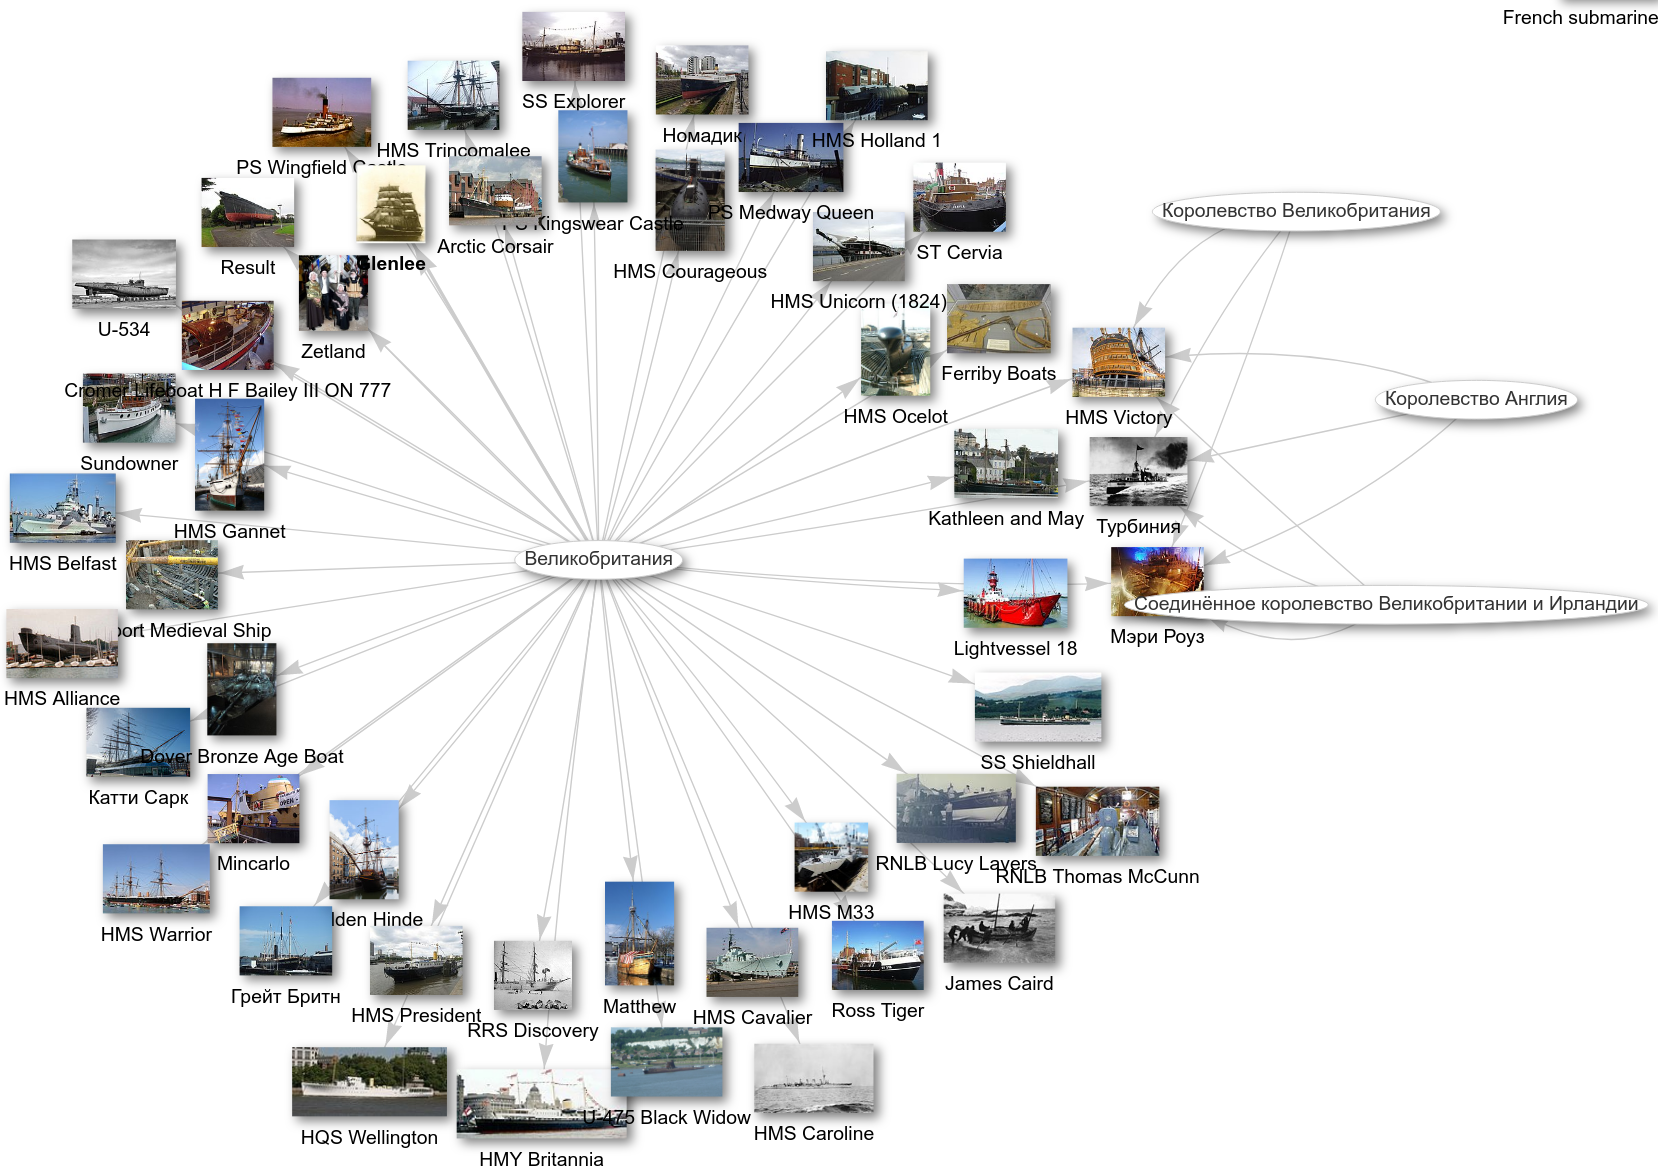
\includegraphics[width=0.9\linewidth]{chapter/ship/double_ring_UK_museum_ships_2024.png}
  \caption{Двойное кольцо кораблей-музеев Великобритании, 
           фрагмент графа стран и~кораблей-музеев, 2024 год}
  \label{fig:double-ring-UK-museum-ships}%
\end{marginfigure}%

\wdqName{Корабль-музей}{575727}~--- это корабль, 
на котором размещена музейная экспозиция, посвященная истории корабля. 
Такие корабли используются в~общеобразовательных и~мемориальных целях. 
Участие корабля в~\wdqName{военном конфликте}{180684} может послужить поводом 
для~создания корабля-музея в~память о~прошедших событиях. 

Чтобы понять большой и~сложный запрос~\ref{lst:museum_graph}, 
рассмотрим сначала строки~21--32 этого запроса как~отдельный скрипт, 
который можно запустить по~ссылке: \href{https://w.wiki/984K}
                                        {https://w.wiki/984K}. 
В~этом фрагменте запроса строятся связи между кораблём-музеем и страной, где расположен музей. 
На рис.~\ref{fig:double-ring-UK-museum-ships} представлен фрагмент графа 
со~страной, имеющей больше всего кораблей-музеев. Конечно, это Великобритания. 



                                        


\newpage
%\begin{minipage}{\linewidth}
\begin{lstlisting}[ language=SPARQL, 
    caption={{\href{https://w.wiki/wz8}
                   {Граф кораблей-музеев и стран, 
                   в которых они находятся (фрагмент скрипта)}}\protect\footnotemark}, 
    label=lst:museum_graph,
    xleftmargin=18pt, 
    numbers=left,
    ]
#defaultView:Graph    
SELECT ?v1 ?v1Label ?v2 ?v2Label ?edgeLabel ?img 
WHERE {
  {SELECT ?c ?cLabel ?v1 ?v1Label ?v2 ?v2Label (STR(COUNT(?c)) as ?edgeLabel) 
   WHERE
   { VALUES ?cTypes 
            {wd:Q180684 # conflict
             wd:Q831663 # military campaign
             wd:Q645883 # military operation
             wd:Q198    # war
            } 
     ?c wdt:P31 ?cTypes.
     ?v1 wdt:P31 wd:Q6256. ?v2 wdt:P31 wd:Q6256. # country
     ?c wdt:P710 ?v1, ?v2. # in war
     FILTER (?v1 != ?v2 && STR(?v1) < STR(?v2)) 
     SERVICE wikibase:label {bd:serviceParam wikibase:language "ru, en"}
  }
  GROUP BY ?c ?cLabel ?v1 ?v1Label ?v2 ?v2Label
  }
 UNION
  {SELECT DISTINCT ?v1 ?v1Label ?v2 ?v2Label ?img
   WHERE
   {
     ?v2 wdt:P31 wd:Q575727. # museum ship
     {?v2 p:P17 [ps:P17 ?v1]} UNION # ?v2 has country ?v1
     {
       ?v2 wdt:P131 ?loc.      # in ?loc
       ?loc p:P17 [ps:P17 ?v1].# ?loc in country ?v1
     } 
     OPTIONAL {?v2 wdt:P18 ?img}
     SERVICE wikibase:label { bd:serviceParam wikibase:language "ru, en"}
   }
 }
}
\end{lstlisting}
%\end{minipage}
\footnotetext{Получено: 117 вершин графа в 2021 году. Ссылка на SPARQL-запрос: \href{https://w.wiki/wz8}{https://w.wiki/wz8}.}


\newpage
%\marginnote[-7.3cm]{%
%
\begin{marginfigure}
%\begin{figure}[h]
  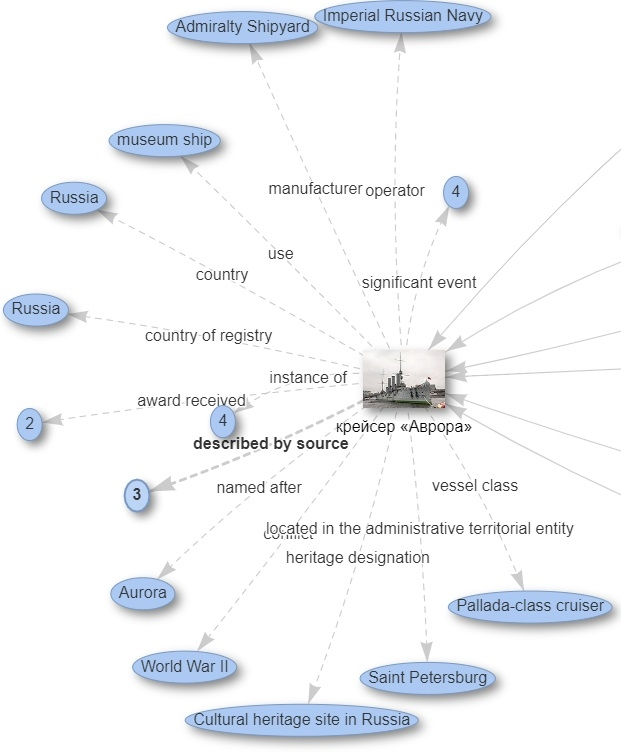
\includegraphics[width=0.83\linewidth]{chapter/ship/aurora_graph_crop.jpg}
  \caption{Граф свойств крейсера <<Аврора>>, 2021 год}%
  \label{fig:aurora_graph}%
%\end{figure}
\end{marginfigure}

Рассмотрим теперь запрос~\ref{lst:museum_graph} в~целом. 
Построим граф кораблей-музеев и воевавших стран 
(рис.~\ref{fig:aurora_graph} и~рис.~\ref{fig:museum_graph}). 
Вершинами графа будут \wdqName{страны}{6256} 
                    и~\wdqName{корабли-музеи}{575727}. 
Ребро между кораблём и~страной означает, что корабль-музей находится в этой стране. 
А ребро между двумя странами означает, 
что эти страны участвовали в одних и тех же конфликтах, число которых равно весу ребра 
(вес подписан на~рёбрах, соединяющих страны). 
Итак, запрос~\ref{lst:museum_graph} строит граф по описанным выше правилам. 

    \index{SPARQL!p:[ps:]!country}
    При определении \emph{страны} для переменных $v1$ и $v2$ 
    посредством свойства \wdProperty{17}{государство} 
    в~строках 25 и 28 запроса~\ref{lst:museum_graph} 
    используется конструкция \texttt{p:/ps:} (точнее: \texttt{\{?v2 p:P17 [ps:P17 ?v1]\}}). 
    Это нужно потому, что у стран в поле 
    \href{https://www.wikidata.org/wiki/Property:P31}{экземпляр (P31)}, 
    кроме значения <<страна>>, могут быть и другие значения. 
    Эта конструкция позволяет перебрать все значения поля P31 и найти значение <<страна>>.
    См.~подробности в главе~\ref{ch:RussiaNotCountryPPS} на с.~\pageref{ch:RussiaNotCountryPPS}.

%}\marginnote[-1.7cm]

Из фрагмента графа на рис.~\ref{fig:museum_graph} видно, 
что корабли-музеи есть у России и~США. 
Эти страны участвовали в~военных конфликтах и они имеют флот, 
а значит, и корабли для создания музеев.


%\begin{figure}[h]
\begin{figure*}[h!]
  \includegraphics[width=0.74\linewidth]{chapter/ship/museum-graph-Russia-USA.png}
  \caption[Граф стран и кораблей-музеев, 2021 год.]
          {Фрагмент графа стран, участвовавших в войнах, и~кораблей-музеев России и США, 2021 год}%
  \label{fig:museum_graph}%
\end{figure*}
%\end{figure}

При просмотре полного графа (и даже на фрагменте, рис.~\ref{fig:museum_graph}) 
видна уникальность научно-иссле\-до\-ва\-тель\-ского судна \wdqName{<<Витязь>>}{1516653}. 
По Викиданным (запрос~\ref{lst:museum_graph}), 
это единственный музей-корабль России, связывающий её с другими странами. 
Изначально этот теплоход был построен и находился на~службе в~Германии, 
что отражено в свойстве <<Витязя>> 
\href{https://www.wikidata.org/wiki/Property:P137}{operator (P137)}=``Кригсма\-рине'' 
(это название военно-морских сил в Третьем рейхе).

Вершины графа на рис.~\ref{fig:museum_graph} кликабельны. 
Например, можно кликнуть на \href{https://www.wikidata.org/wiki/Q168713}{крейсер <<Аврора>> (Q168713)}, 
тогда появятся дополнительные вершины, соответствующие свойствам этого крейсера (рис.~\ref{fig:aurora_graph}).


\section{Упражнения}
\begin{enumerate}
  \item Измените запрос~\ref{lst:museum_graph} так, 
      чтобы граф не содержал вершин-стран без кораблей-музеев. 
  
  \item Измените запрос~\ref{lst:museum_graph} так, чтобы граф содержал 
      только те~страны, которые участвовали больше чем в~одном конфликте.
\end{enumerate}


% last figure
%\begin{figure*}[ht]
%  \includegraphics[width=0.25\linewidth]{chapter/ship/red-green-cells_ships_by_country_and_conflict.png}
%  \caption[Список кораблей и конфликтов, в которых они участвовали]{Фрагмент cписка кораблей, связанных с Россией и участвовавших в военных конфликтах, 2017 год. Из списка видно, что больше большая часть кораблей связаны с Россией и СССР, а также со Второй мировой или Великой Отечественной войнами.}%
%  \label{fig:ships_by_country_and_conflict}%
%\end{figure*}
